%=======================02-713 LaTeX template, following the 15-210 template==================
%
% You don't need to use LaTeX or this template, but you must turn your homework in as
% a typeset PDF somehow.
%
% How to use:
%    1. Update your information in section "A" below
%    2. Write your answers in section "B" below. Precede answers for all 
%       parts of a question with the command "\question{n}{desc}" where n is
%       the question number and "desc" is a short, one-line description of 
%       the problem. There is no need to restate the problem.
%    3. If a question has multiple parts, precede the answer to part x with the
%       command "\part{x}".
%    4. If a problem asks you to design an algorithm, use the commands
%       \algorithm, \correctness, \runtime to precede your discussion of the 
%       description of the algorithm, its correctness, and its running time, respectively.
%    5. You can include graphics by using the command \includegraphics{FILENAME}
%
\documentclass[11pt]{article}
\usepackage{amsmath,amssymb,amsthm}
\usepackage{graphicx}
\usepackage[margin=1in]{geometry}
\usepackage{fancyhdr}
\usepackage{listings}
\usepackage{float} 
\usepackage{subfig}

\setlength{\parindent}{0pt}
\setlength{\parskip}{5pt plus 1pt}
\setlength{\headheight}{13.6pt}
\newcommand\question[2]{\vspace{.25in}\hrule\textbf{#1: #2}\vspace{.5em}\hrule\vspace{.10in}}
\renewcommand\part[1]{\vspace{.10in}\textbf{(#1)}}
\newcommand\algorithm{\vspace{.10in}\textbf{Algorithm: }}
\newcommand\correctness{\vspace{.10in}\textbf{Output: }}
\newcommand\runtime{\vspace{.10in}\textbf{Running time: }}
\pagestyle{fancyplain}
\lhead{\textbf{\NAME\ (\ANDREWID)}}
\chead{\textbf{Project\HWNUM}}
\rhead{\today}
\begin{document}\raggedright
%Section A==============Change the values below to match your information==================
\newcommand\NAME{Yao Xiao}  % your name
\newcommand\ANDREWID{2019180015}     % your andrew id
\newcommand\HWNUM{3}              % the homework number
%Section B==============Put your answers to the questions below here=======================

% no need to restate the problem --- the graders know which problem is which,
% but replacing "The First Problem" with a short phrase will help you remember
% which problem this is when you read over your homeworks to study.

\question{1}{Programming 3} 

\part{a} \algorithm Client
\begin{lstlisting}
# -*-coding:utf-8-*-
import os
import random
import socket
from Crypto.Cipher import AES
from Crypto.Cipher import PKCS1_v1_5 as Cipher_pkcs1_v1_5
import base64
import threading
from Crypto.PublicKey import RSA

# client, server share password
dict = {}
dict["server"] = "12345678"


class prpcrypt():
    def __init__(self, key):
        if len(key) < 16:
            key = key + (16 - len(key)) * "\0"
        self.key = key[:16]
        self.mode = AES.MODE_GCM

    def encrypt(self, text):
        cryptor = AES.new(self.key, self.mode, IV=self.key)
        length = 16
        count = len(text)
        add = count % length
        if add:
            text = text + ('\0' * (length - add))
        self.ciphertext = cryptor.encrypt(text)
        return base64.b64encode(self.ciphertext)

    def decrypt(self, text):
        cryptor = AES.new(self.key, self.mode, IV=self.key)
        plain_text = cryptor.decrypt(base64.b64decode(text))
        return plain_text.rstrip('\0')


def mytarget(connect):

    # authentication
    user = connect.recv(1024)
    if user in dict:
        connect.send("yes")
        pw = dict[user]
        print "user is " + user
    else:
        connect.send("no")
        print "user error"
        connect.close()
        exit(-1)

    # decrypt to get pk 
    ra = connect.recv(1024)
    pc = prpcrypt(pw)
    pk = pc.decrypt(ra)
    print 'pk: ' + pk

    # randomly generate the session key Ks, and send it to the server with double encryption
    a = [random.randint(0, 9) for _ in range(10)]
    Ks = ''.join(str(i) for i in a)
    print "Ks: " + Ks
    rsakey = RSA.importKey(pk)
    cipher = Cipher_pkcs1_v1_5.new(rsakey)
    cipher_text = base64.b64encode(cipher.encrypt(Ks))
    pc = prpcrypt(pw)
    e = pc.encrypt(cipher_text)
    connect.send(e)

    # decrypt NC, randomly generate NS
    data = connect.recv(1024)
    pc = prpcrypt(Ks)
    NC = pc.decrypt(data)
    print 'NC: ' + NC
    a = [random.randint(0, 9) for _ in range(10)]
    NS = ''.join(str(i) for i in a)

    # encrypt NC || NS with Ks and send to server
    NC_B = NC + NS
    pc = prpcrypt(Ks)
    e = pc.encrypt(NC_B)
    connect.send(e)

    # decrypt N2, judge whether N2 is equal to NS
    data = connect.recv(1024)
    pc = prpcrypt(Ks)
    N2 = pc.decrypt(data)
    if N2 == NS:
        print "N2 is equal to NS"
        print "Authentication success"
    else:
        print "Authentication faild"

    while True:
        try:
            data = connect.recv(1024)
        except Exception, e:
            print "User Abnormal Exit"
            exit(-1)
        if data == "quit":
            print "User " + user + " quit!"
            break
        print "User " + user + " say: " + data
        connect.send("receive " + data)
    connect.close()


address = ('127.0.0.1', 8088)
socket = socket.socket(socket.AF_INET, socket.SOCK_STREAM)
socket.bind(address)
socket.listen(5)

while True:
    connect, addr = socket.accept()
    print 'Connected From', addr
    chat = threading.Thread(target=mytarget, args=(connect,))
    chat.start()
\end{lstlisting}

\part{b} \algorithm Server
\begin{lstlisting}
#-*-coding:utf-8-*-
import random
import socket
from Crypto import Random
from Crypto.PublicKey import RSA
from Crypto.Cipher import AES
from Crypto.Cipher import PKCS1_v1_5 as Cipher_pkcs1_v1_5
import base64

# client, server share password
pw = "12345678"

class prpcrypt():
    def __init__(self, key):
        if len(key)<16:
            key=key+(16-len(key))*"\0"
        self.key = key[:16]
        self.mode = AES.MODE_GCM

    def encrypt(self, text):
        cryptor = AES.new(self.key, self.mode, IV=self.key)
        length = 16
        count = len(text)
        add=count % length
        if add:
            text = text + ('\0' * (length-add))
        self.ciphertext = cryptor.encrypt(text)
        return base64.b64encode(self.ciphertext)

    def decrypt(self, text):
        cryptor = AES.new(self.key, self.mode, IV=self.key)
        plain_text = cryptor.decrypt(base64.b64decode(text))
        return plain_text.rstrip('\0')

# random generate
random_generator = Random.new().read
rsa = RSA.generate(1024, random_generator)

# generate pk and sk
pk = rsa.publickey().exportKey()
skS = rsa.exportKey()

address = ('127.0.0.1', 8088)
socket = socket.socket(socket.AF_INET, socket.SOCK_STREAM)
socket.connect(address)

print "pk: " + pk

socket.send('server')
data = socket.recv(1024)
if data == "no":
    print "connect error"
    socket.close()
    exit(-1)

# send pk encrypted with pw
pc = prpcrypt(pw)
e = pc.encrypt(pk)
socket.send(e)

# decrypte to get Ks
data = socket.recv(1024)
pc = prpcrypt(pw)
Ks1 = pc.decrypt(data)
rsakey = RSA.importKey(skS)
cipher = Cipher_pkcs1_v1_5.new(rsakey)
Ks = cipher.decrypt(base64.b64decode(Ks1), random_generator)
print "Ks: " + Ks

# randomly generate NC and send it to client with Ks encryption
a = [random.randint(0,9) for _ in range(10)]
NC = ''.join(str(i) for i in a)
print "NC: " + NC
pc = prpcrypt(Ks)
e = pc.encrypt(NC)
socket.send(e)

data = socket.recv(1024)
pc = prpcrypt(Ks)
N1_2 = pc.decrypt(data)
print 'N1_2: '+N1_2
if N1_2.find(NC) == 0:
    print "Authentication success"
else:
    print "Authentication faild"

# Ks encrypted N2 sent to client
N2 = N1_2[len(NC):]
pc = prpcrypt(Ks)
e = pc.encrypt(N2)
socket.send(e)

while True:
    data = raw_input(">")
    if data == "quit":
        socket.send(data)
        break
    try:
        socket.send(data)
    except Exception, e:
        print "Server Abnormal Exit"
        break
    data = socket.recv(1024)
    print "Server say: " + data
socket.close()
\end{lstlisting}



\part{c} \correctness
\begin{figure}[H]
    \centering
    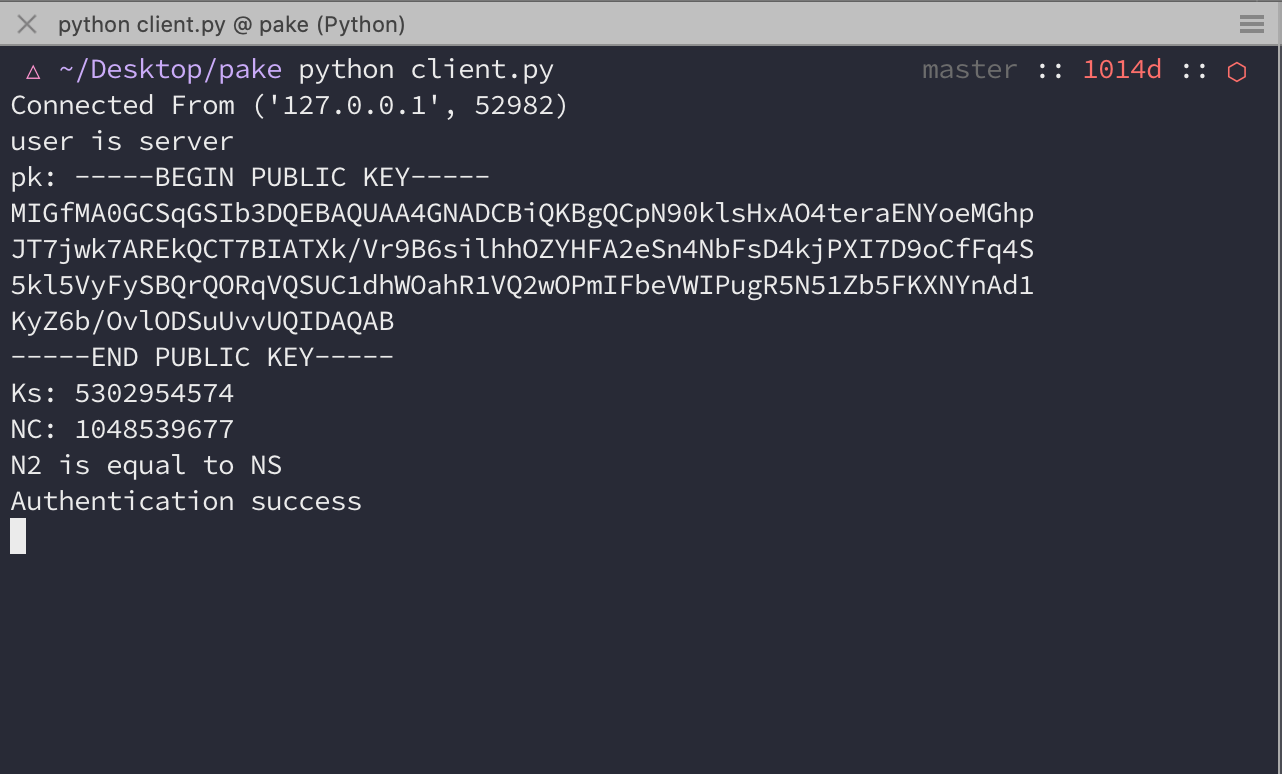
\includegraphics[width=1\textwidth]{client}
    \caption{Client Output}
\end{figure}

\begin{figure}[H]
    \centering
    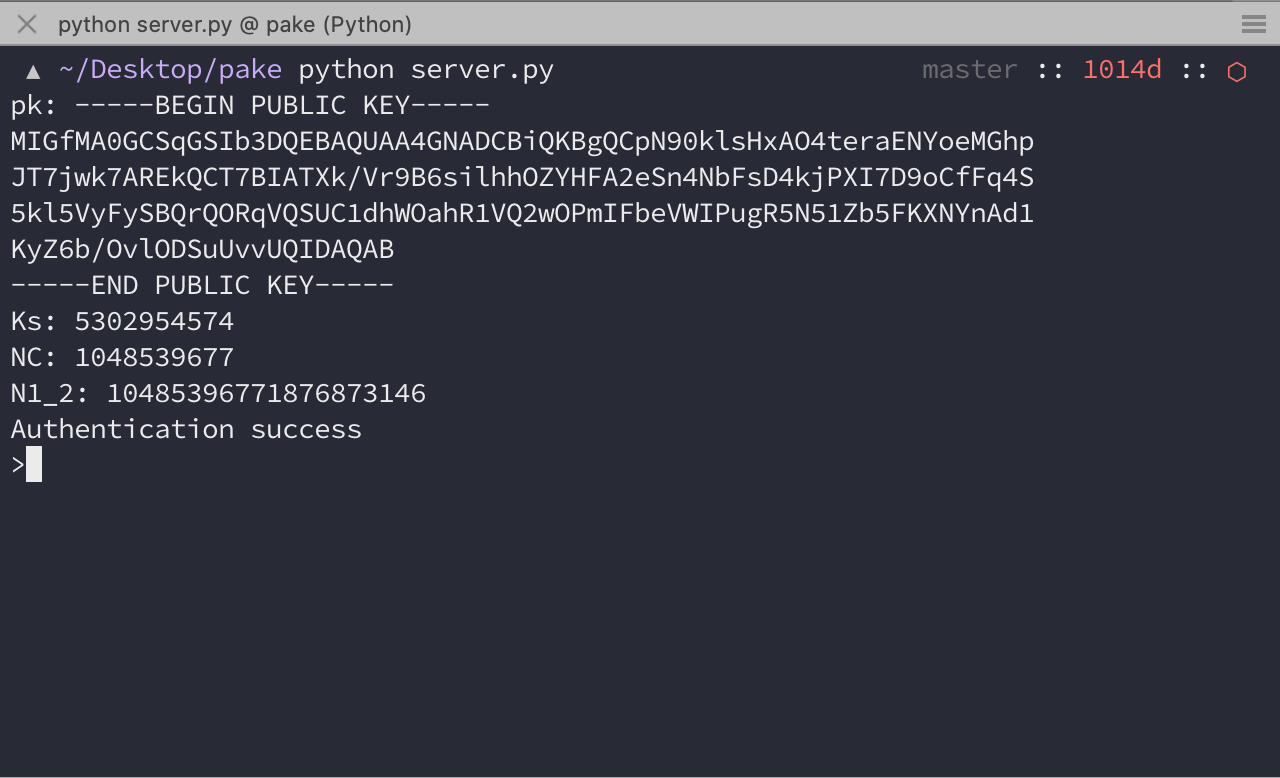
\includegraphics[width=1\textwidth]{server}
    \caption{Server Output}
\end{figure}




\end{document}
